%%%%%%%%%%%%%%%%%%%%%%%%%%%%%%%%%%%%%%%%%
% Minimalist Book Title Page 
% LaTeX Template
% Version 1.0 (27/12/12)
%
% This template has been downloaded from:
% http://www.LaTeXTemplates.com
%
% Original author:
% Peter Wilson (herries.press@earthlink.net)
%
% License:
% CC BY-NC-SA 3.0 (http://creativecommons.org/licenses/by-nc-sa/3.0/)
% 
% Instructions for using this template:
% This title page compiles as is. If you wish to include this title page in 
% another document, you will need to copy everything before 
% \begin{document} into the preamble of your document. The title page is
% then included using \titleTH within your document.
%
%%%%%%%%%%%%%%%%%%%%%%%%%%%%%%%%%%%%%%%%%

%----------------------------------------------------------------------------------------
%	PACKAGES AND OTHER DOCUMENT CONFIGURATIONS
%----------------------------------------------------------------------------------------

%\title{Microprocessor Architecture : Labo 1}

\documentclass{article}

\usepackage[utf8]{inputenc}
\usepackage[T1]{fontenc}
\usepackage[svgnames]{xcolor} % Required to specify font color
\usepackage{mathpazo}
\usepackage{floatrow}
\usepackage{geometry}%réglages mise en page
\geometry{%
a4paper, % note : l'option a4paper tuait la marge supérieure.
body={170mm,250mm}, %
left=25mm,top=25mm,right=25mm, %
headheight=21mm,headsep=7mm,
marginparsep=4mm,
marginparwidth=20mm, %
footnotesep=50mm
}
\usepackage{longtable}
\usepackage{pdflscape}
% allows for temporary adjustment of side margins
\usepackage{chngpage}
\usepackage{graphicx}
\usepackage{float}
\usepackage{color}
\usepackage{amssymb}
\usepackage[hyphens]{url}
\usepackage{hyperref}

\newcommand*{\course}{\fbox{PROJ-H-402}} % Generic publisher logo

%----------------------------------------------------------------------------------------
%	TITLE PAGE
%----------------------------------------------------------------------------------------

\newcommand*{\titleTH}{\begingroup % Create the command for including the title page in the document
\raggedleft % Right-align all text
\vspace*{\baselineskip} % Whitespace at the top of the page

{\Large \textsc{Anthony Debruyn}}\\[0.167\textheight] % Author name

{\LARGE\bfseries Year Project}\\[\baselineskip] % First part of the title, if it is unimportant consider making the font size smaller to accentuate the main title

{\textcolor{Purple}{\Huge Wysiwyd}}\\[\baselineskip] % Main title which draws the focus of the reader

{\Large \textit{Wine cellar management,~~~~~~~~~~ \\almost without management}}\par % Tagline or further description

\vfill % Whitespace between the title block and the publisher

%\vspace*{30\baselineskip} % Whitespace at the bottom of the page

\includegraphics{Images/icon.png}

\vfill

{\large Gaëtan Podevijn \course}\par % Publisher and logo

%\vspace*{5\baselineskip} % Whitespace at the bottom of the page
\endgroup}

%----------------------------------------------------------------------------------------
%	BLANK DOCUMENT
%----------------------------------------------------------------------------------------

\begin{document} 

\thispagestyle{empty}

\titleTH % This command includes the title page

\newpage

\tableofcontents

\newpage

%----------------------------------------------------------------------------------------
%	Introduction
%----------------------------------------------------------------------------------------

\section{Introduction}

Managing something composed of a large number of element can be tedious and complicated, even when you love doing it. This applies to oenologists as well when it comes to organising their wine cellar. This is where Wysiwyd enters the game. The goal of Wysiwyd is to simplify the management of a wine cellar, to allow the oenologists and others to get the most of it.\\

Wysiwyd takes advantages of the new technologies available on the market, such as QR Code scanning and generating, NFC tags, to sort bottles. Photos of the bottles can be captured, so the user can see them right in the app as well. A search can be made on a lot of bottle properties to retrieve a desired bottle. The target OS is Android, leader on the smartphone market. The combination of the discovery of those technologies, the world of Android, the experience gained in mobile programming and design, is what makes this project interesting.\\

These technologies are also what differentiate this app from other wine cellar management apps already available on the market. QR and NFC allow quick retrieval of bottles.

\section{Comparing to other solutions}

What differentiate Wysiwyd from the other applications? In this section this app will be compared to other apps.

\begin{description}
	\item[Vivino] The app Vivino requires an internet connection to work, to recognise a bottle. On the other side, Wysiwyd only uses the local database to get the corresponding bottle and does not work with image recognition, but with QR/bar code or NFC.
	
	\item[Eurocave] Does not offer quick bottle recognition, and presents a lot of bugs, as reported on the Playstore.
	
	\item[Wine Cellar] Does not offer NFC tag functionality. Less properties are editable for a bottle.
	
\end{description}

	Wysiwyd tries answer the needs of oenologists in an ergonomic and aesthetic way.

%----------------------------------------------------------------------------------------
%	The App
%----------------------------------------------------------------------------------------
\newpage
\section{The App}

\begin{quotation}
\center \emph{"What you scan is what you drink."\\ "Wysiwyd"}
\end{quotation}

\subsection{Functionalities}

\subsubsection{App Tour}

Once the app is loaded, the user has to choose between 2 actions. To \emph{scan a tag or a visual code}, or to \emph{list directly all the bottles}. Those 2 actions are symbolised by 2 bottles on the screen (see fig \ref{main_screen}).

\begin{figure}[H]
\begin{center}
	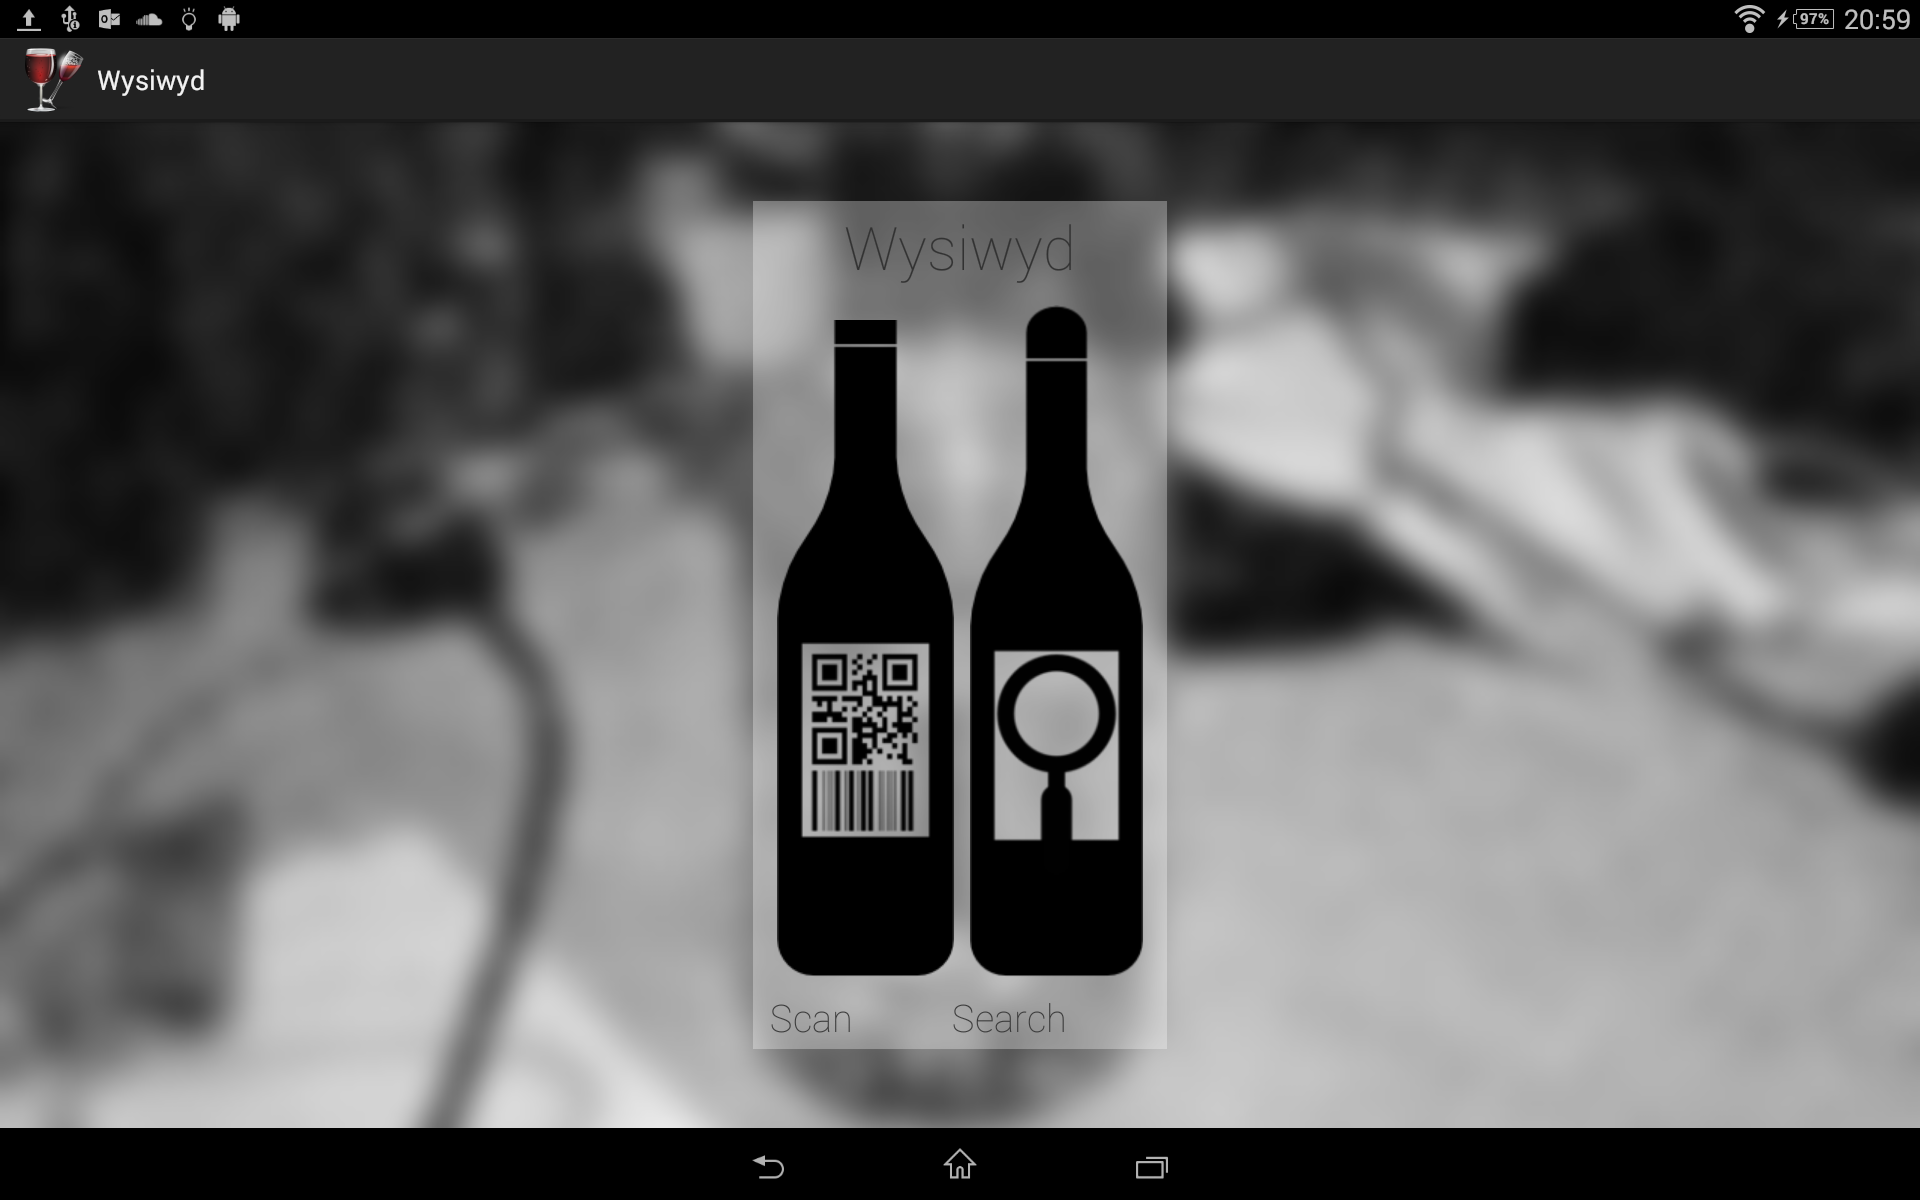
\includegraphics[width=\textwidth]{Images/MainActivity.png}
	\caption{The Main Screen.}
	\label{main_screen}
\end{center}
\end{figure}

If the user touches the first bottle, a new choice pops up: \emph{visual code}, or \emph{NFC tag} scan. This time, it is represented by glasses. The first one opens another app\footnote{Barcode Scanner, by ZXing Team} to scan a bottle bar code, or QR code\footnote{This visual code is the traduction of the number just below the bar code on wine bottles.}. If the user does not have this separate application, he can download it on the playstore for free. This app is not mandatory for this one to work. However, it is highly recommended, as it leads to easier management of the cellar.\\

Behind the glasses, and if the app has at least one image of a bottle, is a blurred picture of a bottle. This picture is one that the user took to illustrate his mobile database.


\begin{figure}[H]
\begin{center}
	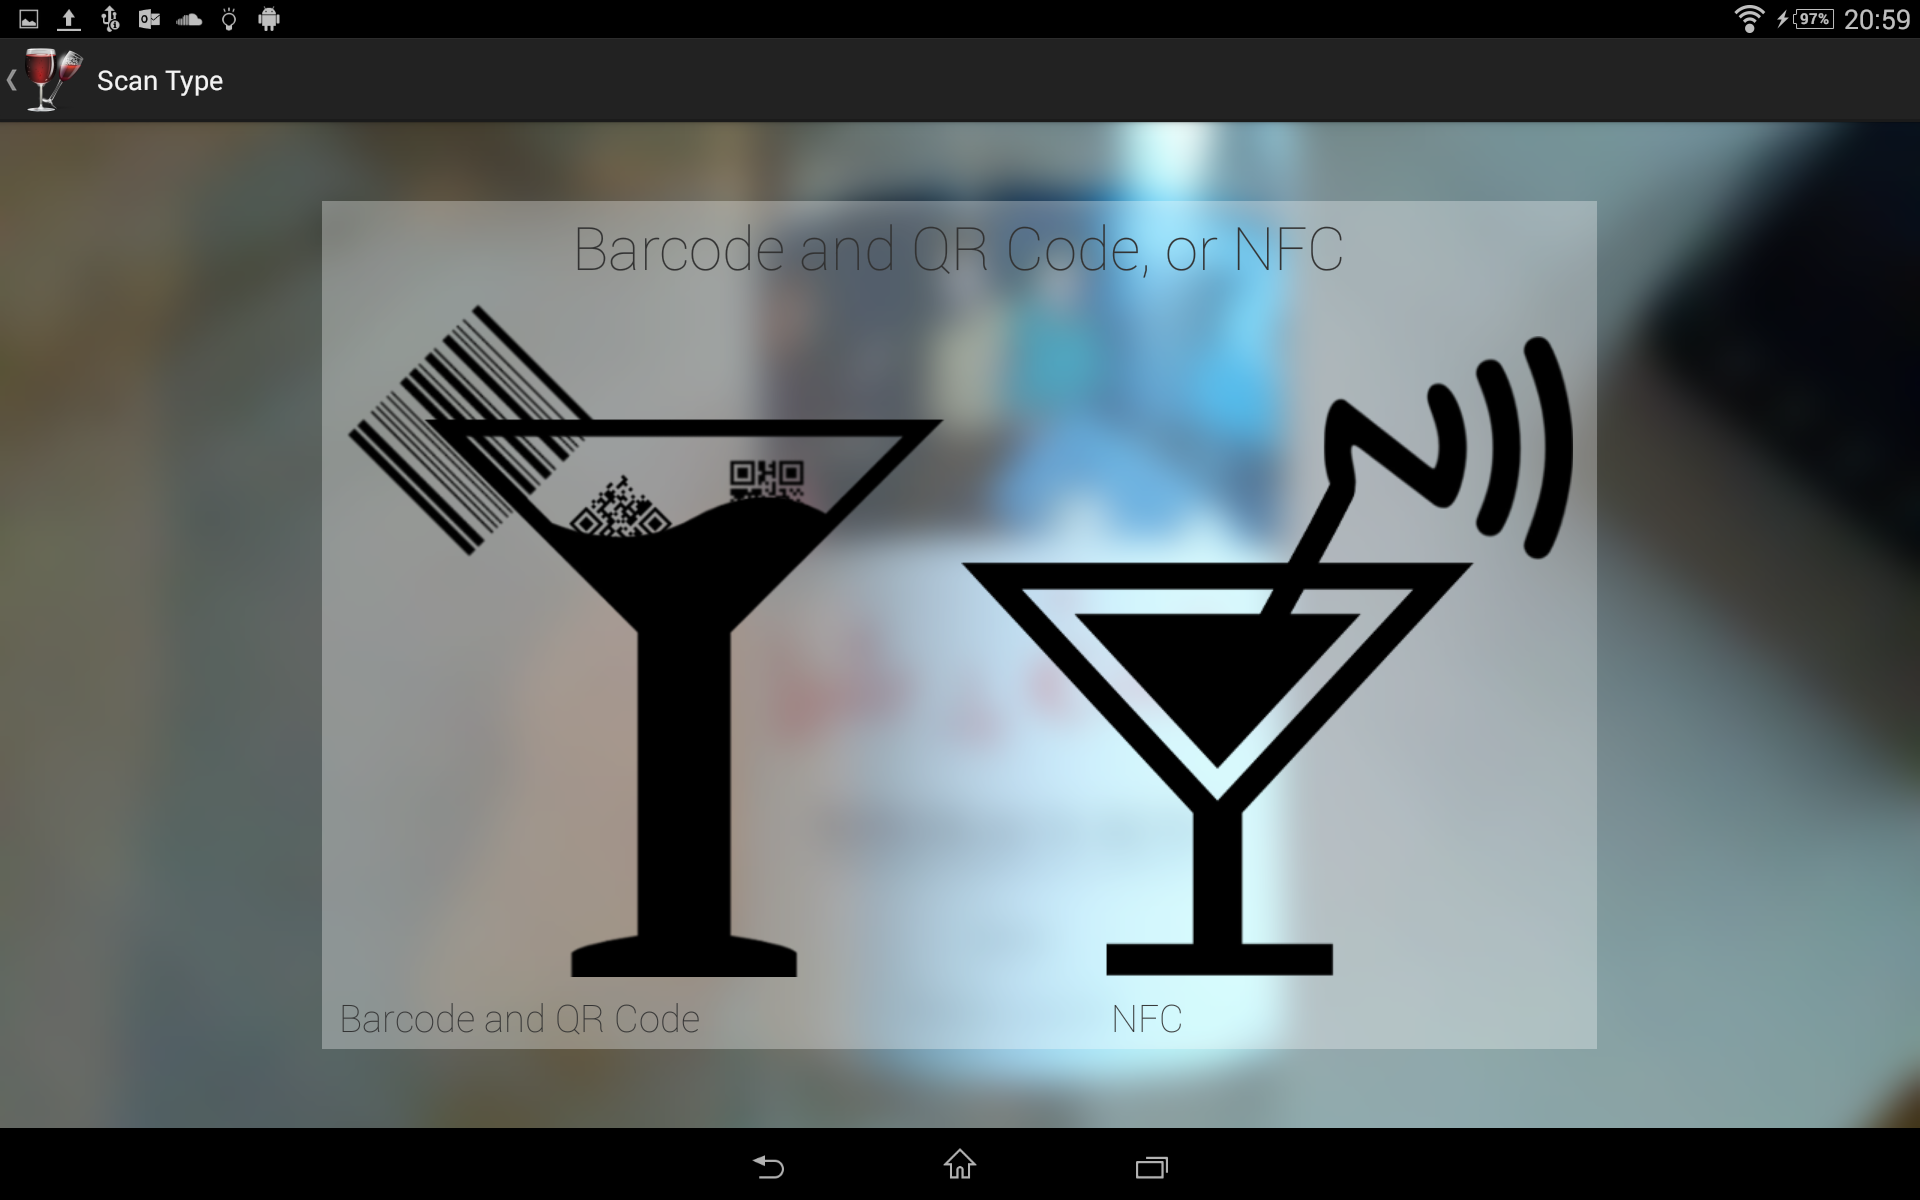
\includegraphics[width=\textwidth]{Images/ScanChoice.png}
	\caption{Visual Code, or NFC Tag ?}
	\label{scan_choice}
\end{center}
\end{figure}

By choosing the second glass, the user arrives in a third screen, only if NFC is available on the device (see fig. \ref{nfc_scan}). The NFC is in foreground mode as long as the user stays in this view. This means that no other app can intercept the NFC tag scan. Of course, if the user is not viewing this screen, the system still can intercept the tag if he places a bottle NFC tag near the NFC ship of the device. Then the system launches the app and directly lists the bottles with the corresponding code.

\begin{figure}[H]
\begin{center}
	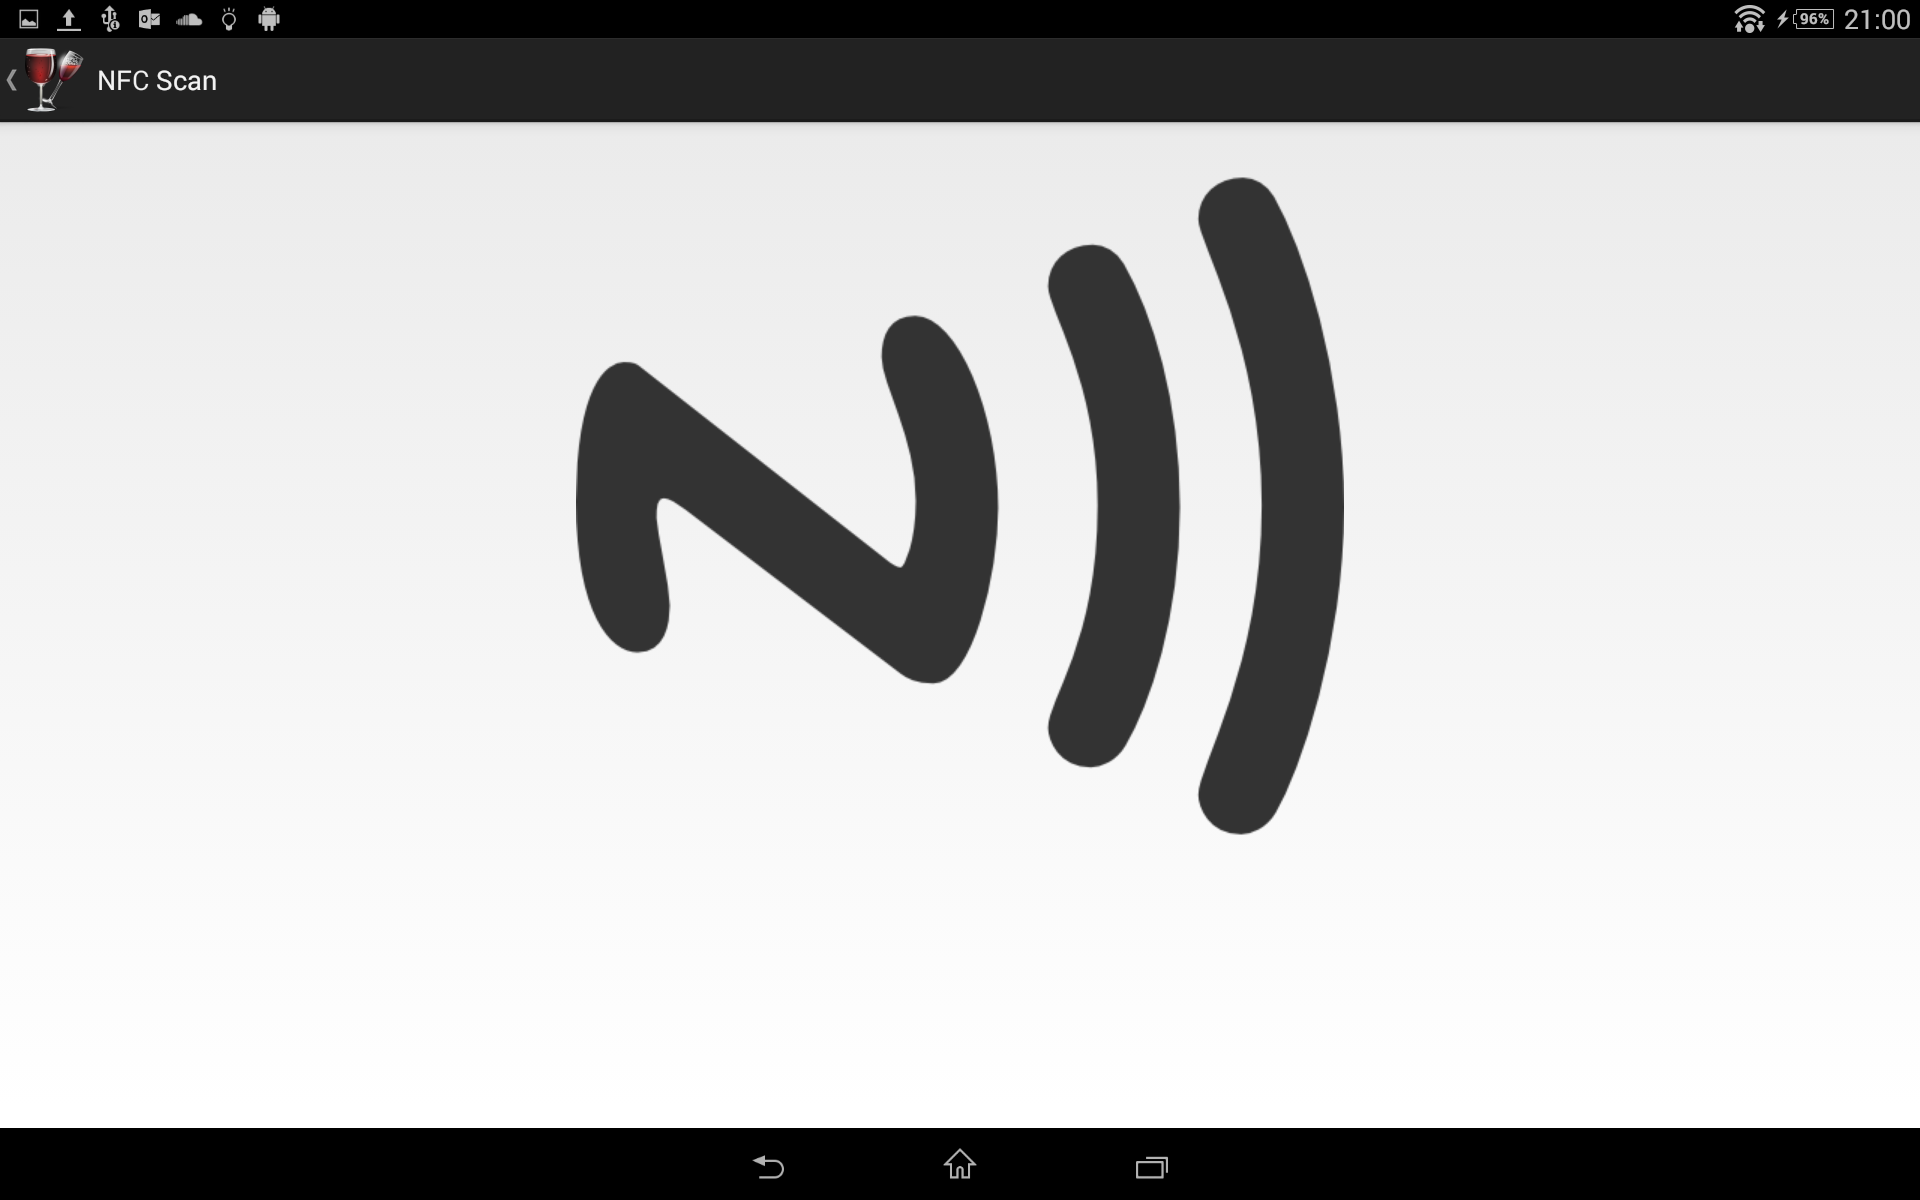
\includegraphics[width=\textwidth]{Images/NFCReaderActivity.png}
	\caption{NFC Tag Scan.}
	\label{nfc_scan}
\end{center}
\end{figure}

When the code has been captured, one way or another, the app shows a list of the corresponding bottles (fig. \ref{list_results}). If the user decides to add a bottle, the code will be copied in the corresponding text field automatically. If on figure \ref{main_screen} the user selected the second bottle, the screen on figure \ref{list_results} opens directly, displaying all the bottles in the order they were added to the database.

\begin{figure}[H]
\begin{center}
	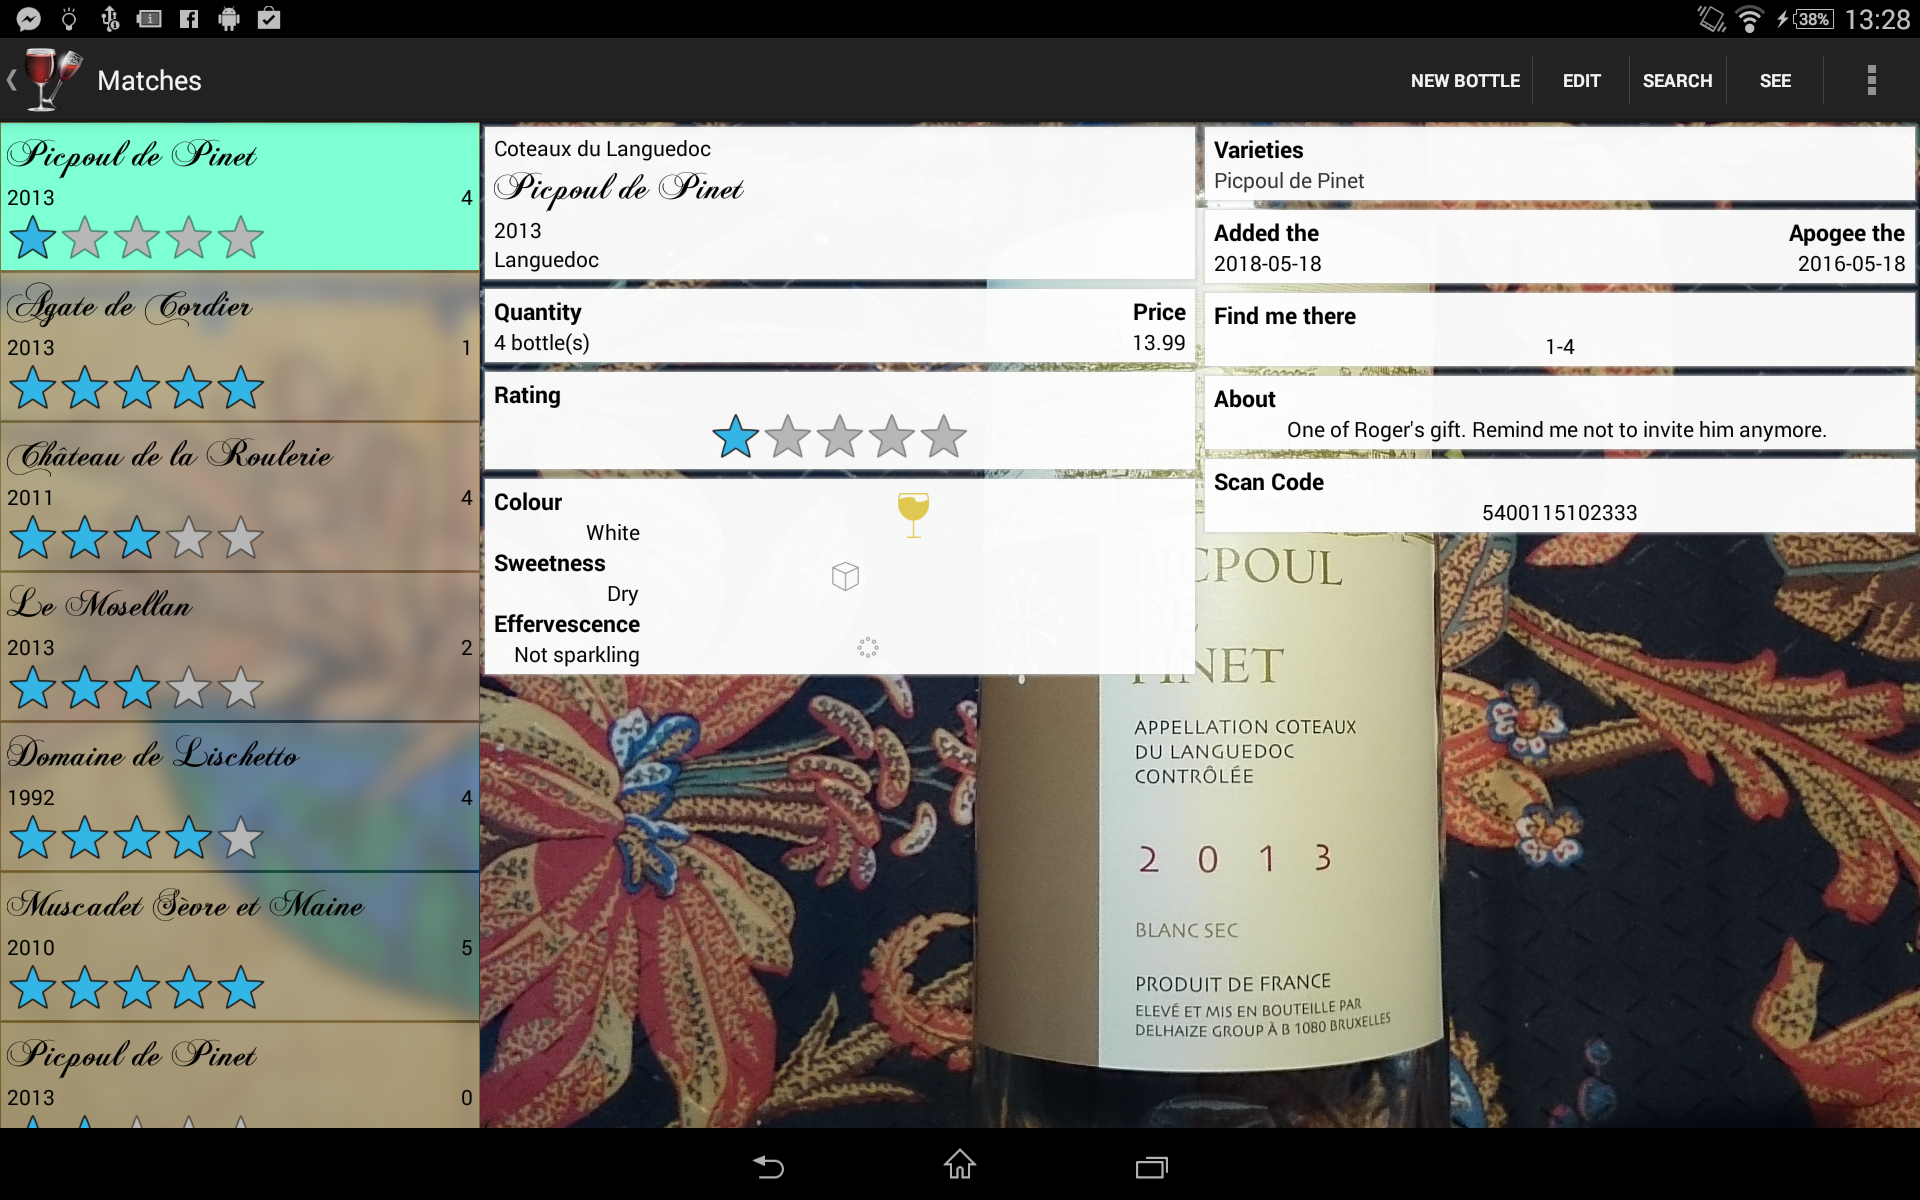
\includegraphics[width=\textwidth]{Images/ResultsActivity.png}
	\caption{List of results.}
	\label{list_results}
\end{center}
\end{figure}

On this figure, one can see all the details about a bottle. This is the view shown on a large screen device. On smaller devices, only one view is displayed at a time, either the details or the list.\\

Several buttons are aligned at the top right of the screen:
\begin{description}
\item[New Bottle:] To create a new bottle. Fill all the necessary text fields and other information, and click on \emph{Done}.
\item[Edit:] To edit an existing bottle. Click on \emph{Done} when finished.
\item[Search:] To search for bottles. Write down the desired properties, and click on \emph{Ok}. The list will refresh to display only the matching bottles.
\item[See:] To see the captured image of the bottle lying behind the view. This hides the details to show the background.
\end{description}

A \emph{long touch on the code section} in the details will open the code exportation functionality. It will allow you to export the code to a QR code or/and to NFC tag. The layout of the corresponding view is similar to the figure \ref{scan_choice}. To generate a QR code and send it, the user is supposed to click on the "QR glass", while to write a NFC tag, the user has to push the "NFC glass" and bring a tag close to the device NFC ship. After generating the QR code, one can send it to a web service like Drive from Google, or email it.

\subsubsection{Adding a Bottle}

There are several ways to add a bottle in the database:

\begin{enumerate}
\item The user \emph{can touch the "search bottle"} on the main screen (fig. \ref{main_screen}), then \emph{touch New Bottle}. This is the preferred method if no visual code is on the bottle, like a bar code or a QR code. If the user wants to add a bottle that has a lot in common with another saved bottle in the database, he can just \emph{keep his finger on that bottle} for a while. After a short time, the new bottle view will appear with all the fields already completed with the information from the previous bottle.

\item If the bottle has a bar/QR code, then the user is advised to go with the scan solution. After the "scan bottle" has been touched, he then chooses the QR/bar code scan. The scan app will open, or a pop up will offer to download it on the Playstore if it is not on the phone. He can now \emph{aim at the printed code} on the bottle with the camera of the device, and wait for the code to be recognised. If the device has no camera, this feature will not be accessible.
\end{enumerate}

\subsubsection{Finding a bottle}

To retrieve a bottle in the database, one can choose between different methods:

\begin{enumerate}
\item If the code of the bottle has been correctly entered in the database, and a NFC tag and/or a bar/QR code is on the bottle, the best option is to \emph{choose the first action} on figure \ref{main_screen}. Then another choice is available to the user to choose between the 2 technologies offered with the app.

\item If no code/tag is on the bottle, or if the user wants to retrieve a bigger amount of bottles matching certain properties, the second action of figure \ref{main_screen} is the best. In the list screen, one can open the search view by \emph{touching Search}.
\end{enumerate}

%----------------------------------------------------------------------------------------
%	The Architecture
%----------------------------------------------------------------------------------------


\section{The Architecture}

\subsection{The Database}

The database used in this project is made with SQLite. The global architecture of the database is simple, as we can see on the entity relationship diagram.

\subsubsection{The Entity Relationship Diagram}

Here is the ERD. The diagram contains 2 entities, linked with a relation. All attributes characterising one bottle are in the Bottle entity, they are not represented by separate entities. This would result in more tables in the database, and more resource consuming queries. Having more tables for these attributes would have been useful if these attributes were changed a lot by the user and if a lot of bottles shared same values for them. Here we supposed that the user will not change these values a lot after entering the bottle information, as the information associated to a bottle of wine rarely change in the market.

\begin{figure}[H]
\begin{center}
	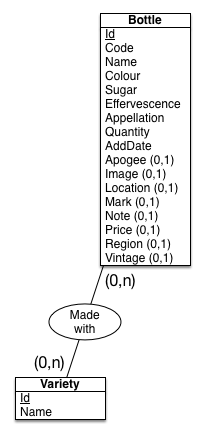
\includegraphics[scale=0.7]{../Entity Relationship DB diagram.png}
	\caption{The ERD. Key is underlined, and optional attributes are together with a (0,1).}
\end{center}
\end{figure}

\paragraph{Constraints}

\begin{itemize}
	\item If the effervescence is 0, then the vintage attribute is mandatory.
	\item Id, Code, Quantity, Vintage are a natural numbers.
	\item Price is a positive real number.
	\item Colour is a natural number in $\{ 0, 1, 2\}$.
	\item Sugar is a natural number in $\{0, 1, 2, 3\}$.
	\item Effervescence is a natural number in $\{0, 1, 2, 3\}$.
	\item Mark is a natural number in $\{1, 2, 3, 4, 5\}$.
	
\end{itemize}

\subsubsection{The Relational Model}

The translation of the ENR into the relational model:

\begin{description}
	\item[Bottle](\underline{Id}, Code, Name, Colour, Sugar, Effervescence, Appellation, Quantity, AddDate, \textit{Apogee}, \textit{Image}, \textit{Location}, \textit{Mark}, \textit{Note}, \textit{Price}, \textit{Region}, \textit{Vintage})
	
	\item[Variety](\underline{Id}, \underline{Name})
	
	\item[BottleVarieties](\underline{Bottle Id, Variety Id})\\ \\
	\emph{BottleVarieties.Bottle Id} foreign key to \emph{Bottle.Id}\\
	\emph{BottleVarieties.IdVariety} foreign key to \emph{Variety.Id}

\end{description}

\paragraph{Constraints}

\begin{itemize}
	\item If the type is "Champagne", then the Year attribute is not mandatory.
	\item The AddDate must be $\leq$ the current date.
	\item Id, Code, Quantity, Vintage are a natural numbers.
	\item Price is a positive real number.
	\item Colour is a natural number in $\{ 0, 1, 2\}$.
	\item Sugar is a natural number in $\{0, 1, 2, 3\}$.
	\item Effervescence is a natural number in $\{0, 1, 2, 3\}$.
	\item Mark is a natural number in $\{1, 2, 3, 4, 5\}$.
	\item For each Bottle Id in BottleVariety, there exists an Id in Bottle.
	\item For each Variety Id in BottleVariety, there exists an Id in Variety.
\end{itemize}

\paragraph{Remark}
Numbers are given to colours, varieties, etc. to allow the use of string resources. This is recommended by the Android best practices, and allows to create multiple versions of the string resources for multiple languages.

\subsubsection{Normalisation}

No normalisation was necessary.

\subsection{The Code}

The implementation of the app was made by trying to respect the best practices in Android application development. All information concerning the UI was stored in xml files (layout files). The hole architecture was thought in an optimisation and object oriented perspective, by taking advantages of the given Android callbacks and life cycle methods.\\

The code is split in several packages. Each package providing a functionality. These packages are described after. Here is the class diagram of the code:
\begin{landscape}
\begin{figure}[H]
\begin{center}
	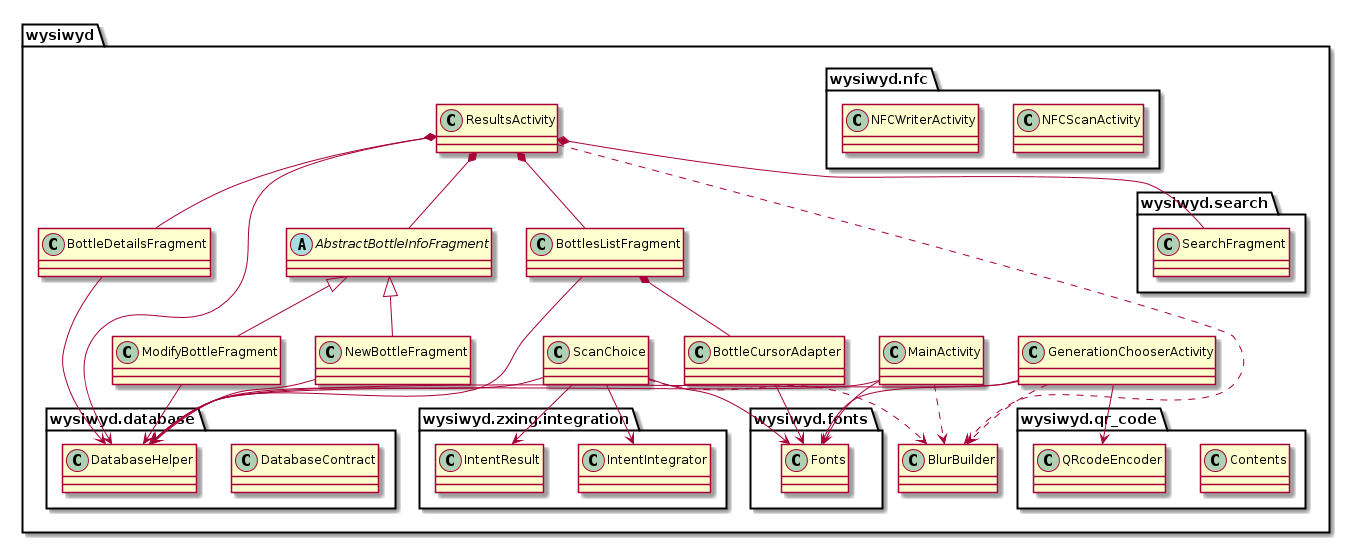
\includegraphics[width=\textwidth]{Images/ClassDiagram.png}
	\caption{The Class Diagram of the code architecture.}
\end{center}
\end{figure}
\end{landscape}
\subsubsection{Root package (wysiwyd)}

The root package (root means the highest level of the src packages hierarchy) contains the main navigation Android activities, from the welcome screen activity to the export chooser for the code exportation. Each situation in the app is associated with another activity in the code.\\

The results activity, the one that shows the list of bottles is special in the sense that it uses fragments. This allows a better modularisation of the code, and easier management of the view. Indeed, 2 modes are currently available in the app, depending on what type of device the app is running on. If the app is run on a large screen device, then the app will use a different layout to take advantage of the screen. 2 fragments will be displayed at the same time: the list and the details/modification/new bottle/search fragment.\\

To be able to communicate with their parent activities, each fragment defines an interface. This interface must be implement by the interface, and this is checked by the fragment each time the fragment is attached to the activity, in the life cycle callback \emph{onAttach}. This interface contains the callbacks methods that are needed by the fragment when it needs to send a message to the activity. As an example, the search fragment has a callback method to give the activity a Bundle object containing all the information needed to build the search query. That way the activity can contact the list fragment, so this latter can build and execute the query.\\

All the information displaying fragment, like the modifying bottle fragment, use callbacks method to save their current state when it is destroyed (not explicitly by the user). This helps reduce resources consumption. It is useful in cases like screen rotation.\\

The use of an abstract class, AbstractBottleInfoFragment, was decided to factorise the code, and take advantage of the polymorphism. This class is inherited by NewBottleFragment and ModifyBottleFragment. These 2 classes have a lot in common, since they both offer tools to specify information on a bottle.

\subsubsection{Database Package (wysiwyd.database)}

The database package contains 2 classes:

\begin{description}
\item[The Contract Class] This class contains the structure of the database, the constants used in other places in the project to build queries, and the strings for the scripts to create the tables.

\item[The Database Helper Class] This class inherits from SQLiteOpenHelper from the Android framework, and is used to get access to the database. A singleton pattern is used in the class to only have one instance of this class created the hole time. This guaranties that no leaks will occur if the access is asked several times. This class also deals with the creation of the database and its upgrade.
\end{description}

\subsubsection{Fonts Package (wysiwyd.fonts)}

Only one class is in this package, and it is used to get access to fonts that are not in the Android framework. A singleton pattern is used for the class, to guarantee that only a single instance will be made.

\subsubsection{NFC Package (wysiwyd.nfc)}

It contains the classes needed to communicate with NFC tags. One class to read and one to write, 2 Android activities. They inherit from classes in an external library (NDEF Tools for Android, see \ref{used_libraries}).

\subsubsection{QR Code Package (wysiwyd.qr\_code)}

Two classes from an external library populate this package (ZXing, see \ref{used_libraries}). These classes are used to communicate with the ZXing library to generate QR codes.

\subsubsection{Search Package (wysiwyd.search)}

Only one class: the search fragment, displayed when the user wants to find a bottle with some properties.

\subsubsection{ZXing Integrator Package (zxing.integration)}

Rather than importing all the code needed to scan visual codes, like QR/bar codes, these 2 classes look for an external application, made by the ZXing developers. This external application is launched each time a scan is needed, and return the result to the calling activity. This way of implementing the code was chosen over the hole importation, since it is easier, and guarantees the last version of the scanning functionality code at all times.

\subsection{Used Libraries}
\label{used_libraries}

\begin{description}
\item[CWAC LoaderEx (commonsguy)] Loaders are a way to load information in a separate thread, and not in the UI thread to avoid lag in the interface. Since the use of loaders was encouraged by the Android best practices, searches were made in that direction. Apparently, the use of loaders with SQLite queries was depreciated, and only their use with content providers was possible. Content providers are useful when it comes to data interaction between applications, and seemed a bit overkill in this app. So an external library was used to compensate this: CWAC LoaderEx from commonsguy. See \url{https://github.com/commonsguy/cwac-loaderex}.

\item[NDEF Tools for Android] This library offers high level programming for NFC communications, as the Android framework does not provide it. This made the implementation of the NFC communication easier, and faster. See \url{https://code.google.com/p/ndef-tools-for-android/}.

\item[ZXing] This is an open-source, multi-format barcode image processing library. Barcodes can also be generated. It was used for the bar code scanning and generating functionalities. See \url{https://github.com/zxing/zxing/}.
\end{description}


%----------------------------------------------------------------------------------------
%	Difficulties
%----------------------------------------------------------------------------------------

\section{Difficulties}

Here are explained the main difficulties met during the implementation of the app.

\begin{description}

	\item[Layout Creation] One of the biggest difficulties encountered was to find the good adjustments for the layout parameters. These parameters, like the weight of a view, the scaling type for an image, the size of views, have to be correctly defined to obtain the desired layout. In xml layout files, like the one for the scan choice activity, the bottle details fragment, this definition of values was made through a process of trial and errors, trying values that theoretically would lead to success. In these files, the nesting of layout made the job more complicated.
	
	\item[Use of 2 Different Screen Sizes] The use of 2 different screen sizes led to addition of code in the results activity. Tests to know in what size it was were added to behave differently. Indeed, different layout files have to be loaded and, in large screen size, some buttons have to be hidden manually. In single pane mode (small screens), these buttons are hidden because the fragment associated to them is hidden. This dual mode also caused problems with the rotation of the screen, since an activity is re-created each time the device configuration changes. This was discovered after some research on the problem, and solutions like using the state saving callback method were exploited.
	
	\item[Finding Help] A lot of search was made to find solutions to the problems found while coding. Some of them did not take long, but others did. Sometimes some solutions had to be mixed to create an adapted solution. See section \ref{references}.
	
	\item[Android] The constant evolution of the mobile OS framework causes some implementations to become depreciated. Alternatives had to be found. External libraries were used, like CWAC LoaderEx, to compensate.
	
	\item[Android Layout Loading System] The view layout of a fragment or activity takes some time to be computed and drawn. In the documentation, it is said that the onViewCreated method is called after its creation, as the method name would suggest. However, it is sometimes not the case, as ImageView's layout are not computed. Their width and height were not computed, and were equal to 0 each time the fragment called this callback method. This prevented the implementation of a bitmap size reducing algorithm to use less resources while drawing bitmaps of the bottles in the background, since these values were needed to get the scale factor.
\end{description}

%----------------------------------------------------------------------------------------
%	Some Ideas for the Future
%----------------------------------------------------------------------------------------

\section{Some Ideas for the Future}

\begin{description}
	\item[Cloud Database] The current database is local, on the device itself. Putting a copy of the database in the cloud would allow the user to use different devices to manage his wine cellar, these devices being synchronised. The user could also share its cellar content with other people. This could be used by shops to offer another view of their stock.
	
	\item[Notification System] A notification system would alert the user that some bottles are going to enter apogee. Another filter could also be based on the apogee criterion in the sorting preference for the results list.
	
	\item[Exportation of the database] The database could be exported to specified file type for consultation on another device. This file could be printed to make a human readable "book" of the content of a wine cellar. Shops could print a catalogue of their cellar content.
	
	\item[Advanced Find Me There Functionality] The information of the location of a bottle could be enhanced. The user could as an example take a picture of the location of the bottle, with a crosshair on the picture denoting the location of the bottle on the picture itself.
	
	\item[Below 4.0 Compatibility] Use the support library to make the code compatible with former Android devices.
	
	\item[Pages in Search Results] Split the results in pages to make the navigation through it easy.
	
	\item[Port to Other Systems] Port the app to other platforms, like iOS, Windows Phone...
\end{description}

%----------------------------------------------------------------------------------------
%	References
%----------------------------------------------------------------------------------------

\section{References}
\label{references}

Here are the links that helped implementing the app by offering solutions:

\subsection{General}

\begin{itemize}
	\item \url{http://developer.android.com/training/index.html} \\The developer training.
	\item \url{http://stackoverflow.com/questions/3769762/android-color-xml-resource-file} \\Contains a lot of predined colors.
	\item \url{http://developer.android.com/guide/index.html} \\Android guide.
	\item \url{http://www.codeproject.com/Articles/525313/Using-Cursor-Loader-in-Android} \\Cursor loaders.
	\item \url{http://www.mkyong.com/android/android-date-picker-example/} \\Date pickers.
	\item \url{http://stackoverflow.com/questions/14445070/difference-between-initloader-and-restartloader-in-loadermanager} \\Difference between initloader and restartloader.
	\item \url{http://stackoverflow.com/questions/18147354/sqlite-connection-leaked-although-everything-closed/18148718#18148718} \\Singleton on the database helper.
	\item \url{http://stackoverflow.com/questions/6750069/get-the-current-fragment-object} \\Retrieve a fragment instance.
\end{itemize}

\subsection{Layout}

\begin{itemize}
	\item \url{http://stackoverflow.com/questions/2025282/difference-between-px-dp-dip-and-sp-in-android} \\To get the different measure units.
	\item \url{http://www.uifuel.com/android-creating-a-drop-shadow-in-xml-layout/} \\To create a dropping shadow around an object.
	\item \url{https://www.grokkingandroid.com/adding-action-items-from-within-fragments/} \\Managing action items programmatically.
	\item \url{http://stackoverflow.com/questions/5179686/restoring-state-of-textview-after-screen-rotation} \\Retaining textview text during configuration change (not activated by default like EditText).
	\item \url{http://www.giantflyingsaucer.com/blog/?p=1342} \\Autocomplete textview powered from SQLite query.
	\item \url{http://etcodehome.blogspot.co.at/2011/05/android-imageview-scaletype-samples.html} Scale type for images in ImageView's.
\end{itemize}

\subsection{Taking Photos}

\begin{itemize}
	\item \url{http://developer.android.com/training/camera/photobasics.html}\\Android guide to capture pictures.
\end{itemize}

\subsection{QR Code}

\begin{itemize}
	\item \url{http://stackoverflow.com/questions/4782543/integration-zxing-library-directly-into-my-android-application/15510698#15510698} \\How to use the QR code generation library.
\end{itemize}

\subsection{Send}

\begin{itemize}
	\item \url{http://stackoverflow.com/questions/4775141/send-email-with-bitmap-object-as-an-attachment-in-android} \\Send a picture.
	\item \url{http://stackoverflow.com/questions/11428189/android-send-an-email-with-an-image-from-an-imageview} \\Send a picture.
\end{itemize}

\subsection{Icons}

Here are references associated to the icons I used to create mine (Gimp).

\begin{itemize}
	\item Bottle, magnifier, bar code, glasses: icons made by Freepik from Flaticon.com.
	\item \url{http://www.psd100.com/nfc-sign-icon/#.U3-1Eh-K-kA} \\NFC tag icon.
\end{itemize}

\subsection{Report}

\begin{itemize}
	\item \url{http://tex.stackexchange.com/questions/49788/hyperref-url-long-url-with-dashes-wont-break} \\To help putting a line break at the right places in the references URLs.
\end{itemize}

\newpage
\section{Special Thanks}
\vfill
\begin{center}
To Gaëtan Podevijn, for providing me with advice, and knowledge on the wine world, throughout the period of the project.\\ ~\\

To my family, for the support, the advices, and the wine bottles used in the tests.\\ ~\\

To Robin Dooreman, for letting me use his smartphone as test device.\\ ~\\

To Quentin Delhaye, for the name of the app.
\end{center}

\vfill
\center 
\includegraphics[width=200px]{Images/icon.png}

\vfill
\end{document}